\documentclass[8pt]{beamer}
\usepackage{graphicx}
\usepackage{xcolor}
\usetheme{default}
\begin{document}
\begin{frame}
\centering
\large{8 TeV MC Closure Test}
\newline
mu\_raw is the number of vertices reconstructed
\newline
mu\_real is the number of vertices after the fake correction has been applied
\newline
mu\_vis is the number of vertices after both corrections have been applied
\end{frame}
\begin{frame}
\center
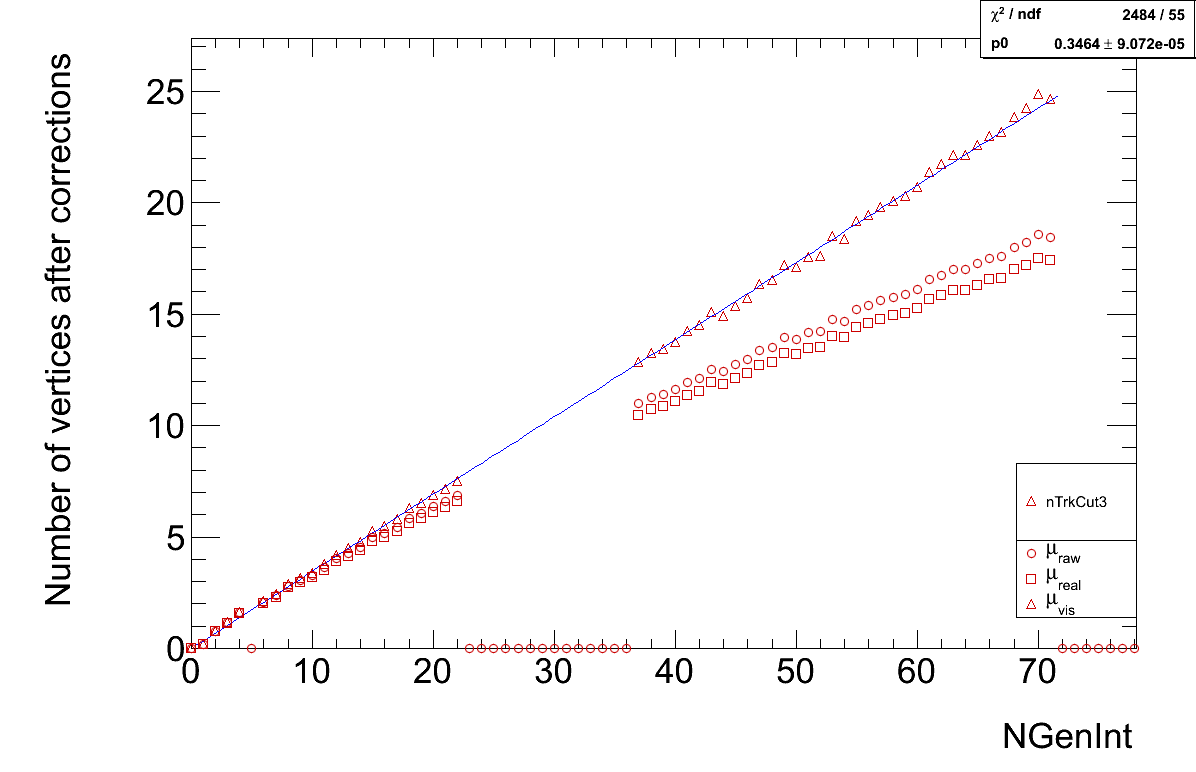
\includegraphics[scale=0.5]{c_muinsteps_ngenint_nTrkCut3}
\end{frame}
\begin{frame}
\center
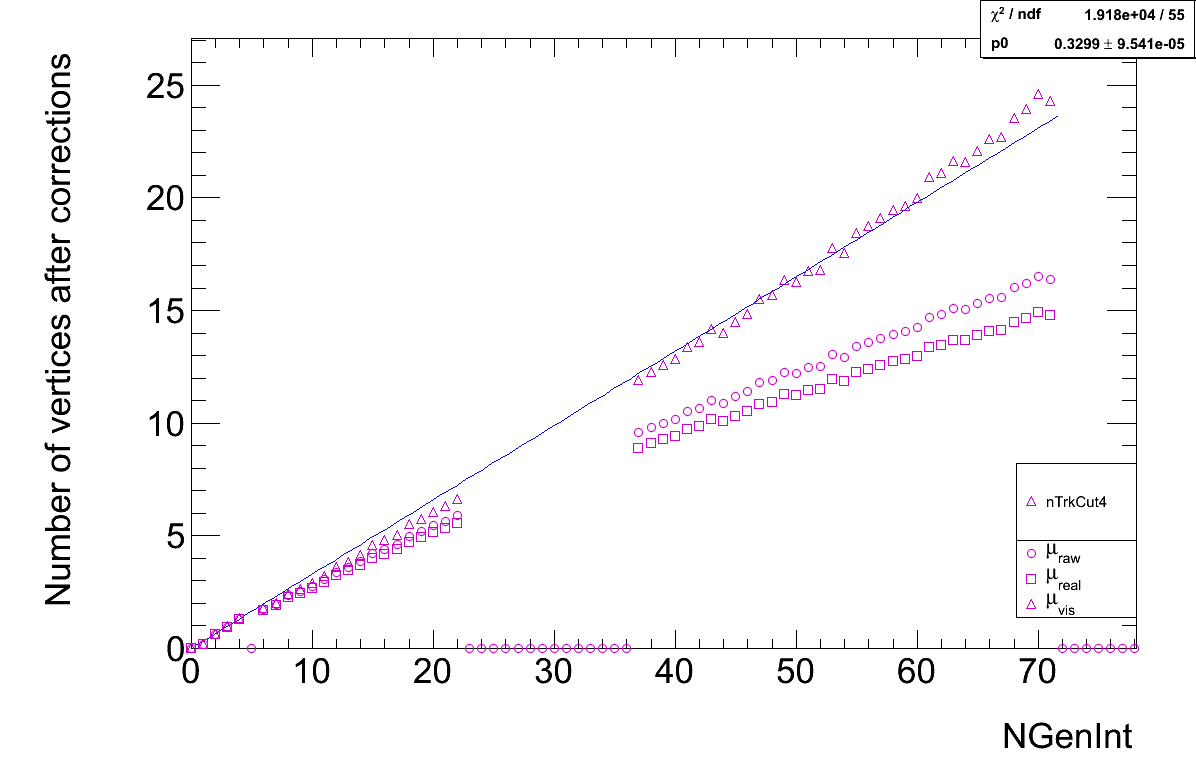
\includegraphics[scale=0.5]{c_muinsteps_ngenint_nTrkCut4}
\end{frame}
\begin{frame}
\center
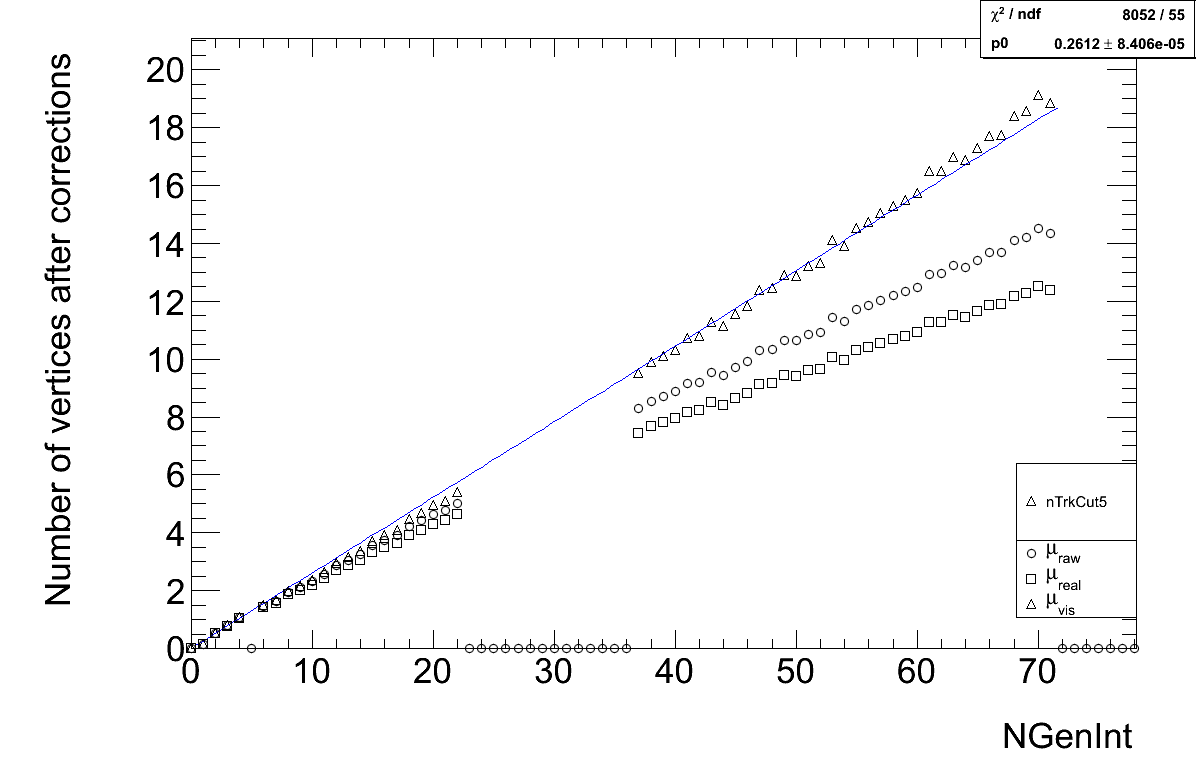
\includegraphics[scale=0.5]{c_muinsteps_ngenint_nTrkCut5}
\end{frame}
\end{document}

